With the verification of Moltres' neutronics modeling capabilities in the
context of the \gls{MSFR}, we now move on to the multiphysics simulation
results. This chapter covers the steady-state multiphysics simulation results
from Moltres.

The procedure for obtaining the steady-state results involved several steps
due to the highly coupled \glspl{PDE}. First, we ran a preliminary transient
simulation of fluid flow in the \gls{MSFR} core, starting from zero inlet
velocity and gradually ramping it up to match the nominal flow rate (4.5 m$^3$
s$^{-1}$); otherwise Moltres had difficulty converging to the desired fully
developed flow profile. We imposed a parabolic flow profile at the inlet.
Next, we imported these fully developed flow values as initial values for
velocity in the actual transient simulation modeling the full coupled
neutronics and thermal-hydraulics. The initial values for the temperature and
neutron group flux distributions are 953 K and $1 \times 10^{14}$ cm$^{-2}$
s$^{-1}$ uniformly throughout the geometry. Finally, we assume that steady
state is reached when the volume integral values of every variable remain
constant (up to 6 sig. fig.) for at least four seconds in the simulation; this
time period corresponds to the nominal circulation time of the \gls{MSFR}.

For a direct comparison with the steady-state results from the Polimi/TUDelft
models, the bulk of our steady-state results do not have decay heat modeling.
Instead, we separately discuss the minor differences borne from decay heat
modeling in the last subsection.

\section{Thermal-Hydraulics}

Figure \ref{fig:flow-temp} shows the temperature and velocity fields
of the fuel salt in the core at steady state from Moltres and the
Polimi/TUDelft models. The results from Moltres show good qualitative
agreement with the Polimi/TUDelft models; we observe similar flow and hotspot
features in all three models. There is a large recirculation region near the
blanket tank walls arising from turbulent flow. Inertial forces dominate over
viscous forces to form this large eddy. The figure also shows two relatively
stagnant regions along the central axis at the top and bottom of the core.
Temperature hotspots form in these regions of recirculation as convection is
the dominant heat transfer mechanism. The maximum temperature from Moltres,
1279 K near the bottom of the recirculation zone, is closer to the maximum
temperature in the Polimi model ($\approx$ 1300 K) than the TUDelft model
($\approx$ 1200K). The minimum temperature is 922 K at the inlet. Figure
\ref{fig:flow} provides an alternate view of the flow profile through flow
streamlines superimposed on the velocity magnitude distribution. The fastest
salt flow occurs at the inlet, outlet, and at core half-height approximately
0.40 m away from the central axis.

\begin{figure}[htb!]
    \centering
    \begin{subfigure}[t]{.37\textwidth}
        \centering
        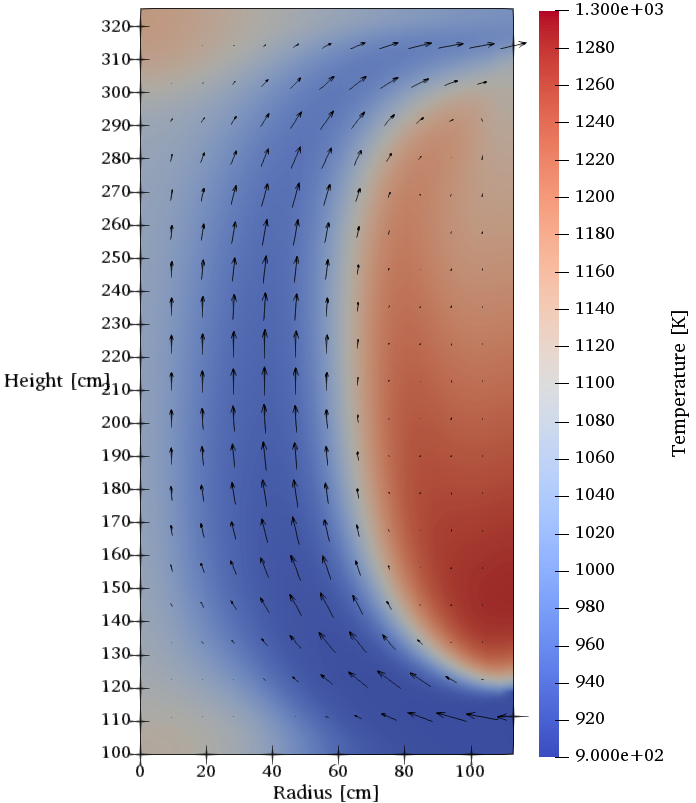
\includegraphics[width=\textwidth]{flow-temp}
    \end{subfigure}
    \hfill
    \begin{subfigure}[t]{.625\textwidth}
        \centering
        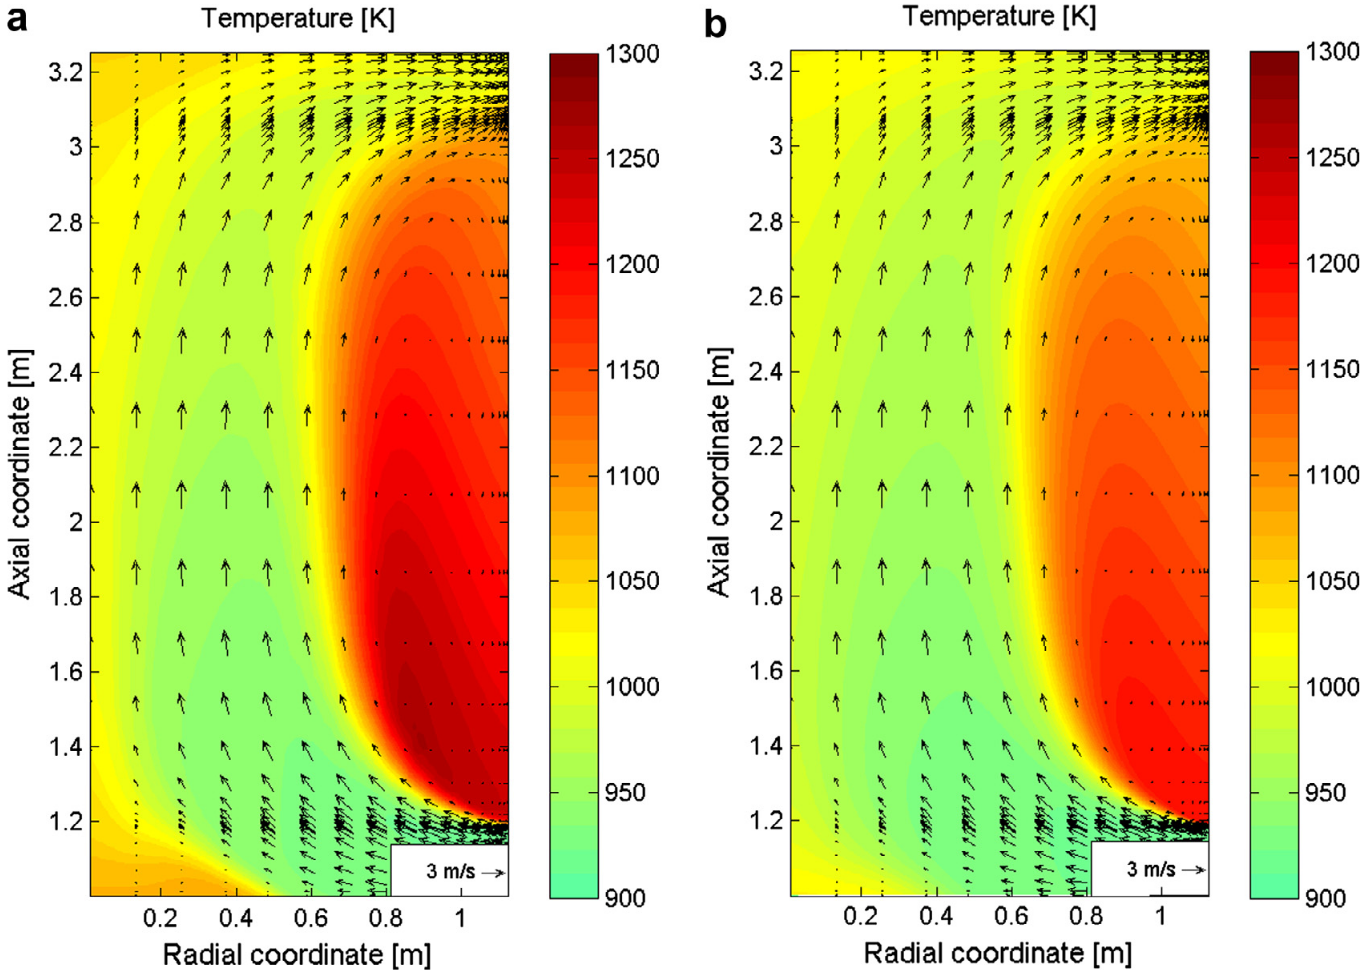
\includegraphics[width=\textwidth]{flow-temp-fiorina}
    \end{subfigure}
    \caption{Temperature and velocity fields in the core from Moltres
    (left), Polimi (center), and TUDelft (right) models. The colors represent
    temperature according to the respective colorbars while the arrows
    represent velocity fields.}
    \label{fig:flow-temp}
\end{figure}

\begin{figure}[htb!]
    \centering
    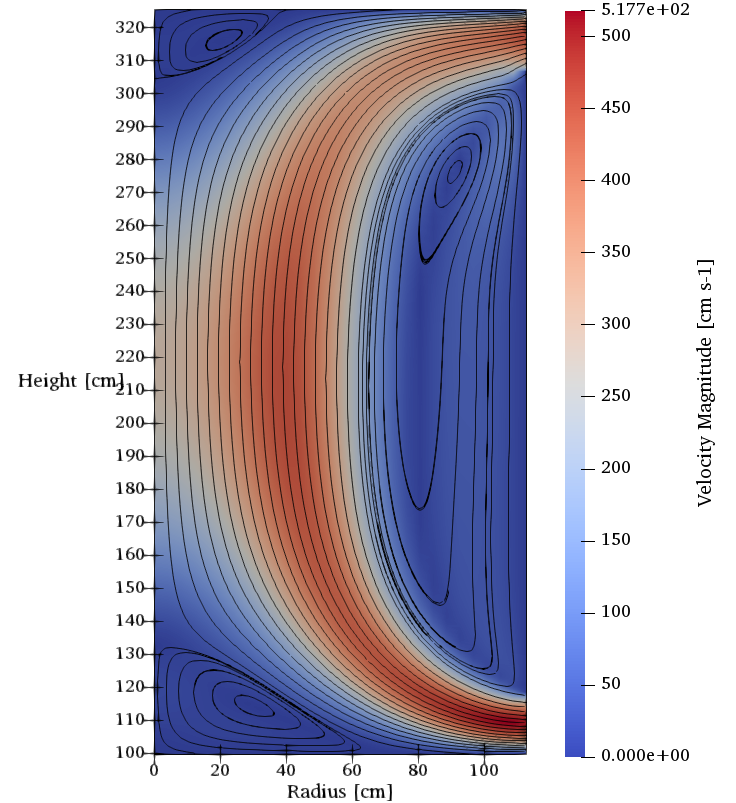
\includegraphics[width=.6\textwidth]{flow}
    \caption{Fuel salt flow streamlines and velocity magnitude in the core.
    The colors represent velocity magnitude according to the colorbar on the
    right.}
    \label{fig:flow}
\end{figure}

While the temperatures at the hotspots are well below the melting point of the
Ni-alloy structure (1500 K), they may cause undue thermal stress on the
blanket tank structure and induce relatively faster salt corrosion rates. A
sudden, large reactivity insertion could push fuel salt temperatures above the
melting point of the Ni-alloy and cause irreversible damage. Furthermore,
the reservoir of hot fuel salt may cause unpredictable behavior during
transient scenarios when the flow profile undergoes a drastic change.
Thus, Rouch et al. \cite{rouch_preliminary_2014} developed an improved
hourglass-shaped design to optimize flow distribution and prevent these
recirculation zones and hotspots from forming. A study of this new design
using Moltres is a potential subject for future work when a proper turbulence
model is in place.

\section{Neutronics}

The neutron flux distribution represents the heat source distribution in a
nuclear reactor. Figure * shows the neutron flux distributions for all six
neutron energy groups. The distribution forms the symmetrical shape we expect
to see in a nuclear reactor with the peak at the center of the core. The
relatively lower temperatures near the center of the core enhances the neutron
flux peak but it is not a major concern as there are no structural parts
vulnerable to neutron damage in that region. The total flux at the center is
*, which is very close to values reported by Fiorina et al. 
\cite{fiorina_molten_2013} and Aufiero \cite{aufiero_development_2014}, albeit
their results are from their neutronics models at a fixed uniform temperature.

\begin{figure}[htb!]
    \centering
%    \includegraphics[width=.6\textwidth]{}
    \caption{Neutron flux distributions in the core for neutron energy groups
    1 to 6.}
    \label{fig:neutronflux}
\end{figure}

As mentioned before, the \glspl{DNP} are mobile in \glspl{MSR} and their
distributions do not directly correspond to the neutron flux distributions.
The location where delayed neutrons are emitted impacts their neutron
importance according to their proximity to fissile and parasitic isotopes.
Figure * shows the \gls{DNP} distributions for all eight \gls{DNP} groups. The
precursors from the shortest-lived group (Group 8) predominantly decay within
the core as their half-lives are shorter than the time it takes to reach the
outlet while the precursors from the longest-lived group (Group 1) are
effectively uniformly distributed due to their long half-lives relative to the
average circulation time. For the longer-lived groups, the mesh elements with
relatively high and low \gls{DNP} concentrations near the outlet and inlet,
respectively, suggest that the mesh is too coarse. Thus, we would recommend
further refinement for future work involving similar geometries.

\begin{figure}[htb!]
    \centering
%    \includegraphics[width=.6\textwidth]{}
    \caption{\gls{DNP} distributions in the core for \gls{DNP} groups
    1 to 8.}
    \label{fig:dnp}
\end{figure}

An important parameter for \gls{MSR} codes is the overall in-core
$\beta_{\text{eff}}$ value. This value represents the true effective delayed
neutron fraction in \glspl{MSR} that accounts for the loss of delayed neutrons
due to \gls{DNP} decay outside the core where fissions cannot be sustained. 
** DNP values and comparison **

\section{Decay Heat}

The inclusion of a decay heat model effectively redistributes a fraction of
the volumetric heat source from the center of the core to the entire loop.
Thus, we expect to observe a slight flattening of the temperature distribution
across the entire primary loop.
